\documentclass[../fem.tex]{subfile}

\begin{document}
\section{Problem}%
\label{sec:problem}

\subsection{Setup}%
\label{sub:setup}

For this problem, we consider the matrices that define the $L$ operator to be
\begin{align*}
  A=\begin{bmatrix}
    1 & 0\\ 0 & 1
  \end{bmatrix}\qquad
  B=\begin{bmatrix}
    0 \\ 0
  \end{bmatrix}\qquad
  C=0.
\end{align*}
Thus we can write the operator $L$ to be
\begin{align*}
  L=\ppder{}{x}+\ppder{}{y}.
\end{align*}

\subsection{Problem Statement}%
\label{sub:problem_statement}

We will consider a problem that is time independent, and so will have no time
derivative. This means that the formulation of the problem statement will be
\begin{align*}
  Lu=f.
\end{align*}

The problem that we consider is
\begin{align}
  \ppder{u}{x}+\ppder{u}{y}=-8\sin(2x)\sin(2y).
\end{align}
With the boundary conditions defined by
\begin{align*}
  \partial u(x, y, t)=\sin(2x)\sin(2y).
\end{align*}

\subsection{Analytical}%
\label{sub:analytical}

This problem was specially constructed such that the solution is
\begin{align*}
  u=\sin(2x)\sin(2y),
\end{align*}
we will verify that this is indeed a solution to the problem.

\begin{align*}
  \ppder{}{x}\left[\sin(2x)\sin(2y)\right]&+\ppder{}{y}\left[\sin(2x)\sin(2y)\right]\\
                                          &=\pder{}{x}\left[-2\cos(2x)\sin(2y)\right]+\pder{}{y}\left[-2\sin(2x)\cos(2y)\right]\\
                                          &=-4\sin(2x)\sin(2y)-4\sin(2x)\sin(2y)\\
                                          &=-8\sin(2x)\sin(2y).
\end{align*}
Thus we have proven that a solution to this problem is $u=\sin(2x)\sin(2y)$.

\subsection{Implementation}%
\label{sub:implementation}

We have constructed the finite element analysis, to accept a \texttt{Lua}
script file. The Lua script defines all of the necessary information for the
finite element analysis to proceed. For this problem, we define the problem Lua
script below.

\code{lua}{snippets/r1.lua}

The exact source code for the different settings can be found in the
appendix (Appendix \ref{app:example_source_code}).

\subsection{Unit Square}%
\label{sub:unit_square}

First, we provide the findings on the unit square. We will compare the results
of the unit square on four different mesh resolutions. These resolutions are
$0.25$, $0.1683$, $0.0866$, $0.005$. Recall that the mesh resolution is the maximum
area of the individual triangles of the mesh. We will denote the mesh
resolution using $\mu$. The results of the computations are provided below.

\begin{figure}[htpb]
  \centering
  \begin{subfigure}{0.4\textwidth}
    \centering
    
\includegraphics[width=0.8\linewidth]{figures/r1/tri.png}
    \caption{$\mu=0.25$, $n=13$}
  \end{subfigure}
  \begin{subfigure}{0.4\textwidth}
    \centering
    
\includegraphics[width=0.8\linewidth]{figures/r2/tri.png}
    \caption{$\mu=0.1683$, $n=25$}
  \end{subfigure}
  \begin{subfigure}{0.4\textwidth}
    \centering
    
\includegraphics[width=0.8\linewidth]{figures/r3/tri.png}
    \caption{$\mu=0.0866$, $n=46$}
  \end{subfigure}
  \begin{subfigure}{0.4\textwidth}
    \centering
    
\includegraphics[width=0.8\linewidth]{figures/r4/tri.png}
    \caption{$\mu=0.005$, $n=666$}
  \end{subfigure}
  \caption{Triangular meshes of $\Box^2$ used for solving the problem.}
  \label{fig:b2_mesh}
\end{figure}

\begin{figure}[htpb]
  \centering
  \begin{subfigure}{0.5\textwidth}
    \centering
    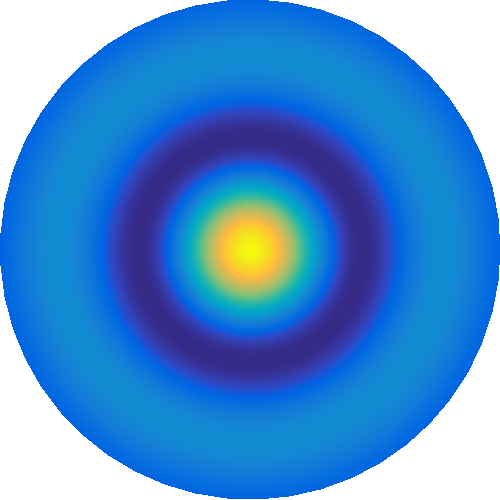
\includegraphics[width=0.8\linewidth]{figures/r1/func.png}
    \caption{Analytical Solution}
  \end{subfigure}

  \begin{subfigure}{0.4\textwidth}
    \centering
    \includegraphics[width=0.8\linewidth]{figures/r1/approx.png}
    \caption{$\mu=0.25$}
  \end{subfigure}
  \begin{subfigure}{0.4\textwidth}
    \centering
    \includegraphics[width=0.8\linewidth]{figures/r2/approx.png}
    \caption{$\mu=0.1683$}
  \end{subfigure}
  \begin{subfigure}{0.4\textwidth}
    \centering
    \includegraphics[width=0.8\linewidth]{figures/r3/approx.png}
    \caption{$\mu=0.0866$}
  \end{subfigure}
  \begin{subfigure}{0.4\textwidth}
    \centering
    \includegraphics[width=0.8\linewidth]{figures/r4/approx.png}
    \caption{$\mu=0.005$}
  \end{subfigure}
  \caption{Side by side comparison of the analytical and numerical solutions.}
  \label{fig:r1_soln}
\end{figure}

It can clearly be seen in figure \ref{fig:r1_soln}, that there is little to no
difference, between the analytical and the numerical solutions, when we have a
higher number of triangles. The very low resolution mesh produces a poor
approximation of the solution. The quantitative comparisons of the different
methods are provided in table \ref{tab:r1}.

\begin{table}[htpb]
  \centering
  \caption{Times and error required for each of the mesh refinement levels.}
  \label{tab:r1}
  \begin{tabular}{c c}
    \begin{tabular}{r l}
      \multicolumn{2}{c}{$\mu=0.25$}\\\hline\hline
      Stage & Time\\\hline
      Mesh & 0.002955\\
      Matrices & 0.076755\\
      Forcing & 0.001223\\
      Solving & 0.000310\\\hline
      Total & 0.081243\\
      Error & 0.378112\\\hline
    \end{tabular}
    &
    \begin{tabular}{r l}
      \multicolumn{2}{c}{$\mu=0.1683$}\\\hline\hline
      Stage & Time\\\hline
      Mesh & 0.004742\\
      Matrices & 0.171679\\
      Forcing & 0.002330\\
      Solving & 0.001908\\\hline
      Total & 0.180689\\
      Error & 0.355618\\\hline
    \end{tabular}\\[2cm]
    \begin{tabular}{r l}
      \multicolumn{2}{c}{$\mu=0.0866$}\\\hline\hline
      Stage & Time\\\hline
      Mesh & 0.002942\\
      Matrices & 0.328250\\
      Forcing & 0.005008\\
      Solving & 0.012522\\\hline
      Total & 0.348722\\
      Error & 0.135833\\\hline
    \end{tabular}
    &
    \begin{tabular}{r l}
      \multicolumn{2}{c}{$\mu=0.005$}\\\hline\hline
      Stage & Time\\\hline
      Mesh & 0.014961\\
      Matrices & 5.650480\\
      Forcing & 0.082520\\
      Solving & 41.652458\\\hline
      Total & 47.400419\\
      Error & 0.010363\\\hline
    \end{tabular}
  \end{tabular}
\end{table}

\subsection{Unit Disk}%
\label{sub:unit_disk}

Now we provide the findings on the unit disk. For the solution on the unit
disk, we decided to impose that the boundary conditions should be zero. This
means that we do not have an analytical solution for this problem, but it
demonstrates the ability for this implementation to handle the boundary
conditions that are imposed. We will compare the results on the unit disk using
the same changes that we made for the unit square. The results of the
computations are provided below.

\begin{figure}[htpb]
  \centering
  \begin{subfigure}{0.4\textwidth}
    \centering
    
\includegraphics[width=0.8\linewidth]{figures/c1/tri.png}
    \caption{$\mu=0.25$, $n=78$}
  \end{subfigure}
  \begin{subfigure}{0.4\textwidth}
    \centering
    
\includegraphics[width=0.8\linewidth]{figures/c2/tri.png}
    \caption{$\mu=0.1683$, $n=80$}
  \end{subfigure}
  \begin{subfigure}{0.4\textwidth}
    \centering
    
\includegraphics[width=0.8\linewidth]{figures/c3/tri.png}
    \caption{$\mu=0.0866$, $n=84$}
  \end{subfigure}
  \begin{subfigure}{0.4\textwidth}
    \centering
    
\includegraphics[width=0.8\linewidth]{figures/c4/tri.png}
    \caption{$\mu=0.005$, $n=525$}
  \end{subfigure}
  \caption{Triangular meshes of $D^2$ used for solving the problem.}
  \label{fig:d2_mesh}
\end{figure}

\begin{figure}[htpb]
  \centering
  \begin{subfigure}{0.4\textwidth}
    \centering
    \includegraphics[width=0.8\linewidth]{figures/c1/approx.png}
    \caption{$\mu=0.25$}
  \end{subfigure}
  \begin{subfigure}{0.4\textwidth}
    \centering
    \includegraphics[width=0.8\linewidth]{figures/c2/approx.png}
    \caption{$\mu=0.1683$}
  \end{subfigure}
  \begin{subfigure}{0.4\textwidth}
    \centering
    \includegraphics[width=0.8\linewidth]{figures/c3/approx.png}
    \caption{$\mu=0.0866$}
  \end{subfigure}
  \begin{subfigure}{0.4\textwidth}
    \centering
    \includegraphics[width=0.8\linewidth]{figures/c4/approx.png}
    \caption{$\mu=0.005$}
  \end{subfigure}
  \caption{Side by side comparison of the analytical and numerical solutions.}
  \label{fig:d1_soln}
\end{figure}

It can clearly be seen in figure \ref{fig:d1_soln}, that there is little to no
difference, between the analytical and the numerical solutions. This is
especially true for the higher refinement of the mesh. The quantitative
comparisons of the different methods are provided in table
\ref{tab:c1}.

\begin{table}[htpb]
  \centering
  \caption{Times and error required for each of the mesh refinement levels.}
  \label{tab:c1}
  \begin{tabular}{c c}
    \begin{tabular}{r l}
      \multicolumn{2}{c}{$\mu=0.25$}\\\hline\hline
      Stage & Time\\\hline
      Mesh & 0.002221\\
      Matrices & 0.470592\\
      Forcing & 0.006835\\
      Solving & 0.053815\\\hline
      Total & 0.533463\\\hline
    \end{tabular}
    &
    \begin{tabular}{r l}
      \multicolumn{2}{c}{$\mu=0.1683$}\\\hline\hline
      Stage & Time\\\hline
      Mesh & 0.005639\\
      Matrices & 0.492630\\
      Forcing & 0.007343\\
      Solving & 0.059259\\\hline
      Total & 0.564871\\\hline
    \end{tabular}\\[2cm]
    \begin{tabular}{r l}
      \multicolumn{2}{c}{$\mu=0.0866$}\\\hline\hline
      Stage & Time\\\hline
      Mesh & 0.002169\\
      Matrices & 0.539801\\
      Forcing & 0.007560\\
      Solving & 0.067315\\\hline
      Total & 0.616845\\\hline
    \end{tabular}
    &
    \begin{tabular}{r l}
      \multicolumn{2}{c}{$\mu=0.005$}\\\hline\hline
      Stage & Time\\\hline
      Mesh & 0.005591\\
      Matrices & 4.446052\\
      Forcing & 0.064099\\
      Solving & 20.156721\\\hline
      Total & 24.672463\\\hline
    \end{tabular}
  \end{tabular}
\end{table}

Clearly for the simple cases like this one, the method of finite element
analysis works extremely well, and quickly for smaller numbers of triangles.

For both of these case increasing the mesh refinement, greatly increased the
number of vertices. The number of vertices is on the order
of$\sim\frac{3}{\mu}$. This means that as $\mu$ is decreased the number of
vertices explodes. This will indicate that the time required for computation
will also explode.

We observe that the time of computation does indeed directly correlate the
number of vertices in the mesh, and is on the order of $\sim N^3$. This means
that a small decrease in mesh size means that the time will grow greatly,
making the approximation take significantly longer to compute.

Finally, we note that the Error term began decreasing slowly, then decreased
very rapidly. If we were to continue with finer meshes, we would see that the
error term would continue to decrease, but the rate at which it would do so
would also be decreasing. We can approximate a graph of what one might expect
of the error term with respect to the number of vertices in the mesh in Figure
\ref{fig:error_decrease}.

\begin{figure}[htpb]
\begin{center}
\begin{tikzpicture}[scale=1, transform shape]
  \begin{axis}[axis lines=middle, xmin=-0.1, xmax=10.1, ymin=-0.1, ymax=1.1,
    yticklabels={,,}, xticklabels={,,}, xlabel=$\mu$, ylabel=$E$]
    \plot[domain=-0.1:10.1]{1/(1+exp(-x+6))};
  \end{axis}
\end{tikzpicture}
\end{center}
\caption{Plot of potential error term.}
\label{fig:error_decrease}
\end{figure}

The shape of the error plot in figure \ref{fig:error_decrease}, can be
considered to be a very generalized shape. As the value of $\mu\rightarrow 0$,
then the error term converges to zero. This means that if one were to use an
indignantly small mesh, then the solution would be exact. The demonstrates that
our implementation is valid, and the error decreases in a manner which we
expect it to.

With this analysis of the implementation, it is clear that larger meshes should
be avoided as much as possible, as they result in drastically longer computation
times. For problems with few changes are very well handled by this method, and
do not require a very fine mesh. However, problems with many changes will be
handled poorly and will require extremely small mesh triangles. This can be
considered in reference to a 2D example.

Consider $\sin(x)$ and $\sin(10x)$, because of the higher frequency of
$\sin(10x)$ it would be less well approximated, without many many triangles,
but $\sin(x)$ would be very easily approximated with only a few triangles. So
with a ``higher frequency'' function a finer mesh would be required to achieve
acceptable error.

\end{document}
